\documentclass[11pt, letterpaper]{report}
%basic packages
\usepackage[utf8]{inputenc}
\usepackage[T1]{fontenc}
\usepackage{graphicx}
\usepackage[margin=0.75in]{geometry}
\usepackage[usenames,dvipsnames]{xcolor}

%math
\usepackage{amsmath, amsthm, amsfonts, amssymb, mathtools}
\usepackage{mathrsfs}
\usepackage{cancel}
\usepackage{siunitx} %phyjsicsssss
\usepackage{bbm} %mathbb for numbers
\usepackage[all]{xy} % https://texdoc.org/serve/xyguide.pdf/0
\makeatletter
\renewcommand*\env@matrix[1][c]{\hskip -\arraycolsep
  \let\@ifnextchar\new@ifnextchar
  \array{*\c@MaxMatrixCols #1}}
\makeatother %matrix realignment

%misc
\usepackage{float}
\usepackage[hyphens]{url}
%\definecolor{page}{HTML}{242526}
%\pagecolor{page}
\usepackage{booktabs} %the \toprule and \bottomrule thick lines on tables

\usepackage{hyperref}
\definecolor{aqua}{HTML}{00C5FF}
\hypersetup{
    colorlinks,
    linkcolor={aqua},
    urlcolor={aqua},
    citecolor={red}
}

%my commands
\DeclarePairedDelimiter\bra{\langle}{\rvert} %Bra
\DeclarePairedDelimiter\ket{\lvert}{\rangle} %Ket
\DeclarePairedDelimiterX\braket[2]{\langle}{\rangle}{#1\,\delimsize\vert\,\mathopen{}#2} %Bra-ket
\newcommand{\pvec}[1]{\vec{#1}\mkern2mu\vphantom{#1}} % from https://tex.stackexchange.com/questions/120029/how-to-typeset-a-primed-vector
\newcommand{\hati}{\boldsymbol{\hat{\textbf{\i}}}}
\newcommand{\hatj}{\boldsymbol{\hat{\textbf{\j}}}}
\newcommand{\hatk}{\boldsymbol{\hat{\textbf{k}}}}
\newcommand{\R}{\mathbb{R}}
\DeclareMathOperator{\diag}{diag}

%theorems
\usepackage{thmtools}
\usepackage{tikz}
\usepackage{tikz-cd}
\usepackage[framemethod=TikZ]{mdframed}
\mdfsetup{skipabove=1em,skipbelow=0em, innertopmargin=5pt, innerbottommargin=6pt}
\theoremstyle{definition} %because obviously
% THEOREM STYLES

\definecolor{boxColor}{HTML}{3D3D3D}

% Definitions
\newcounter{def}[chapter]\setcounter{def}{0}
\renewcommand{\thedef}{\arabic{chapter}.\arabic{def}}
\newenvironment{definition}[1][]{
  \refstepcounter{def}
  \ifstrempty{#1}{
    \mdfsetup{
      frametitle = {
        \tikz[baseline=(current bounding box.east),outer sep=0pt]
        \node[anchor=east,rectangle,font=\bfseries,fill=white]{\strut Definition~\thedef};}}}
  {\mdfsetup{
      frametitle={
        \tikz[baseline=(current bounding box.east),outer sep=0pt]
        \node[anchor=east,rectangle,font=\bfseries,fill=white]{\strut Definition~\thedef :~#1};}}}
  \mdfsetup{innertopmargin=-5pt,linewidth=1pt,topline=true,nobreak,frametitleaboveskip=\dimexpr-12pt\relax\strutbox}
\begin{mdframed}[]}{\end{mdframed}}

% Theorems
\newcounter{thm}[chapter]\setcounter{thm}{0}
\renewcommand{\thethm}{\arabic{chapter}.\arabic{thm}}
\newenvironment{theorem}[1][]{
  \refstepcounter{thm}
  \ifstrempty{#1}{
    \mdfsetup{
      frametitle = {
        \tikz[baseline=(current bounding box.east),outer sep=0pt]
        \node[anchor=east,rectangle,font=\bfseries,fill=white,draw,thick]{\strut Theorem~\thethm};}}}
  {\mdfsetup{
      frametitle={
        \tikz[baseline=(current bounding box.east),outer sep=0pt]
        \node[anchor=east,rectangle,font=\bfseries,fill=white,draw,thick]{\strut Theorem~\thethm~(#1)};}}}
  \mdfsetup{innertopmargin=2pt,linewidth=1pt,topline=true,nobreak,frametitleaboveskip=\dimexpr-13pt\relax\strutbox}
\begin{mdframed}[]}{\end{mdframed}}

% Lemmas
\newcounter{lma}[chapter]\setcounter{lma}{0}
\renewcommand{\thelma}{\arabic{chapter}.\arabic{lma}}
\newenvironment{lemma}[1][]{
  \refstepcounter{lma}
  \ifstrempty{#1}{
    \mdfsetup{
      frametitle = {
        \tikz[baseline=(current bounding box.east),outer sep=0pt]
        \node[anchor=east,rectangle,font=\bfseries,fill=white,draw,thick]{\strut Lemma~\thelma};}}}
  {\mdfsetup{
      frametitle={
        \tikz[baseline=(current bounding box.east),outer sep=0pt]
        \node[anchor=east,rectangle,font=\bfseries,fill=white,draw,thick]{\strut Lemma~\thelma~(#1)};}}}
  \mdfsetup{innertopmargin=2pt,linewidth=1pt,topline=true,nobreak,frametitleaboveskip=\dimexpr-13pt\relax\strutbox}
\begin{mdframed}[]}{\end{mdframed}}


% Corollaries
\newcounter{corr}[chapter]\setcounter{corr}{0}
\renewcommand{\thecorr}{\arabic{chapter}.\arabic{corr}}
\newenvironment{corollary}[1][]{
  \refstepcounter{corr}
  \ifstrempty{#1}{
    \mdfsetup{
      frametitle = {
        \tikz[baseline=(current bounding box.east),outer sep=0pt]
        \node[anchor=east,rectangle,font=\bfseries,fill=white,draw,thick]{\strut Corollary~\thecorr};}}}
  {\mdfsetup{
      frametitle={
        \tikz[baseline=(current bounding box.east),outer sep=0pt]
        \node[anchor=east,rectangle,font=\bfseries,fill=white,draw,thick]{\strut Corollary~\thecorr~(#1)};}}}
  \mdfsetup{innertopmargin=2pt,linewidth=1pt,topline=true,nobreak,frametitleaboveskip=\dimexpr-13pt\relax\strutbox}
\begin{mdframed}[]}{\end{mdframed}}

% Propositions
\newcounter{prp}[chapter]\setcounter{prp}{0}
\renewcommand{\theprp}{\arabic{chapter}.\arabic{prp}}
\newenvironment{proposition}[1][]{
  \refstepcounter{prp}
  \ifstrempty{#1}{
    \mdfsetup{
      frametitle = {
        \tikz[baseline=(current bounding box.east),outer sep=0pt]
        \node[anchor=east,rectangle,font=\bfseries,fill=white,draw,thick]{\strut Proposition~\theprp};}}}
  {\mdfsetup{
      frametitle={
        \tikz[baseline=(current bounding box.east),outer sep=0pt]
        \node[anchor=east,rectangle,font=\bfseries,fill=white,draw,thick]{\strut Proposition~\theprp~(#1)};}}}
  \mdfsetup{innertopmargin=2pt,linewidth=1pt,topline=true,nobreak,frametitleaboveskip=\dimexpr-13pt\relax\strutbox}
\begin{mdframed}[]}{\end{mdframed}}

% Remarks
\newenvironment{remark}[1][]{
  \mdfsetup{
      frametitle={
        \tikz[baseline=(current bounding box.east),outer sep=0pt]
        \node[anchor=east,rectangle,font=\bfseries,fill=white]{\strut Remark};}}
  \mdfsetup{innertopmargin=-7pt,linewidth=1pt,topline=true,bottomline=true,leftline=false,rightline=false,nobreak,frametitleaboveskip=\dimexpr-12pt\relax\strutbox}
\begin{mdframed}[]}{\end{mdframed}}

% Examples
\newenvironment{example}[1][]{
  \mdfsetup{
      frametitle={
        \tikz[baseline=(current bounding box.east),outer sep=0pt]
        \node[anchor=east,rectangle,font=\bfseries,fill=white,draw,thick]{\strut Example};}}
  \mdfsetup{innertopmargin=0pt,linewidth=1pt,topline=true,bottomline=true,leftline=false,rightline=false,nobreak,frametitleaboveskip=\dimexpr-13pt\relax\strutbox}
\begin{mdframed}[]}{\end{mdframed}}

% As Previously Seen
\newenvironment{prev}[1][]{
  \mdfsetup{
      frametitle={
        \tikz[baseline=(current bounding box.east),outer sep=0pt]
        \node[anchor=east,rectangle,font=\bfseries,fill=white]{\strut As Previously Seen};}}
  \mdfsetup{innertopmargin=-7pt,linewidth=1pt,topline=true,bottomline=true,leftline=false,rightline=false,nobreak,frametitleaboveskip=\dimexpr-12pt\relax\strutbox}
\begin{mdframed}[]}{\end{mdframed}}

% Exercises
\newcounter{exe}[chapter]\setcounter{exe}{0}
\renewcommand{\theexe}{\arabic{chapter}.\arabic{exe}}
\newenvironment{exercise}[1][]{
  \refstepcounter{exe}
  \mdfsetup{
      frametitle={
        \tikz[baseline=(current bounding box.east),outer sep=0pt]
        \node[anchor=east,rectangle,font=\bfseries,fill=white,draw,thick]{\strut Exercise~\theexe};}}
  \mdfsetup{roundcorner=10pt,innertopmargin=0pt,linewidth=1pt,topline=true,nobreak,frametitleaboveskip=\dimexpr-13pt\relax\strutbox}
\begin{mdframed}[]}{\end{mdframed}}

%theorem styles
\declaretheoremstyle[headfont=\bfseries, bodyfont=\normalfont, mdframed={linewidth=1pt,   bottomline=false, topline=false, rightline=false}, qed=\(\blacksquare\)]{proofline}
\declaretheoremstyle[headfont=\bfseries, bodyfont=\normalfont, mdframed={linewidth=1pt,   bottomline=false, topline=false, rightline=false}, qed=\qedsymbol]{egline}

\declaretheorem[numbered=no, name=Notation]{notation}

%solution environment
\declaretheorem[numbered=no, style=egline, name=Solution]{setsolution}
\newenvironment{solution}[1][]{\vspace{-10pt}\begin{setsolution}}{\end{setsolution}}
%proof environment
\declaretheorem[numbered=no, style=proofline, name=Proof]{replacementproof}
\renewenvironment{proof}[1][\proofname]{\begin{replacementproof}}{\end{replacementproof}}

% Side Indented Theorems - https://tex.stackexchange.com/questions/429339/shifting-newtheorem
\newtheoremstyle{side}{}{}{\advance\leftskip3cm\relax\itshape\normalfont}{-4pt}
{\bfseries}{}{0pt}{
\makebox[0pt][r]{
  \smash{\parbox[t]{2.5cm}{\raggedright\thmname{#1}.
  \thmnote{\newline(#3)}}}
  \hspace{10.1pt}}}

\theoremstyle{side}
\newtheorem{note}{Note}
\newtheorem{intuition}{Intuition}
\newtheorem{claim}{Claim}
\theoremstyle{definition}

%pulls lecture files
\newcommand{\lec}[2]{%
	\foreach \c in {#1,...,#2}{%
		\IfFileExists{Lectures/lec_\c.tex} {%
			\input{Lectures/lec_\c.tex}%
		}{}%
	}%
}
%to use, in the same file directory as your header.tex and master.tex files, create a folder titled "Lectures" and put your
%lectures into their, named lec_1.tex, lec_2.tex, and so on. In the master.tex file, write \lec{a}{b} where a is the lowest
%number you want to call, and b is the highest.

%fancy headers
\usepackage{fancyhdr}
\pagestyle{fancy}
\fancyhead{}\fancyfoot{}
\fancyfoot[R]{\thepage}
\fancyfoot[C]{\leftmark}


%figures, taken from (https://castel.dev/post/lecture-notes-2)
\usepackage{import}
\usepackage{xifthen}
\usepackage{pdfpages}
\usepackage{transparent}
\newcommand{\incfig}[1]{%
    \def\svgwidth{\columnwidth}
    \import{./figures/}{#1.pdf_tex}
}

%lectures, taken from (https://castel.dev/post/lecture-notes-3)
\makeatother
\def\@lecture{}%
\newcommand{\lecture}[3]{%
	\ifthenelse{\isempty{#3}}{%

		\def\@lecture{Lecture #1}%
	}{%
		\def\@lecture{Lecture #1: #3}
	}
	\subsection*{\@lecture}
	\hfill{\small\textsf{#2}}\par
}
\makeatletter

\author{Grant Talbert}

\usepackage{titlepageBU}
\title{Honors Differential Equations}
\date{09/23/24}
\courseID{MA 231}
\professor{Dr. Eugene Wayne}
\courseSection{A1}
\usepackage{graphicx}
\graphicspath{{./}}
\usepackage{pgfplots}
\newenvironment{soln}[1][]{\noindent\textbf{Solution. }}{\hfill\qedsymbol}
\usepackage{listings}
\begin{document}
\makeproblem
\section*{Section 1.3 Problem 7}
\begin{soln}
\begin{center}
		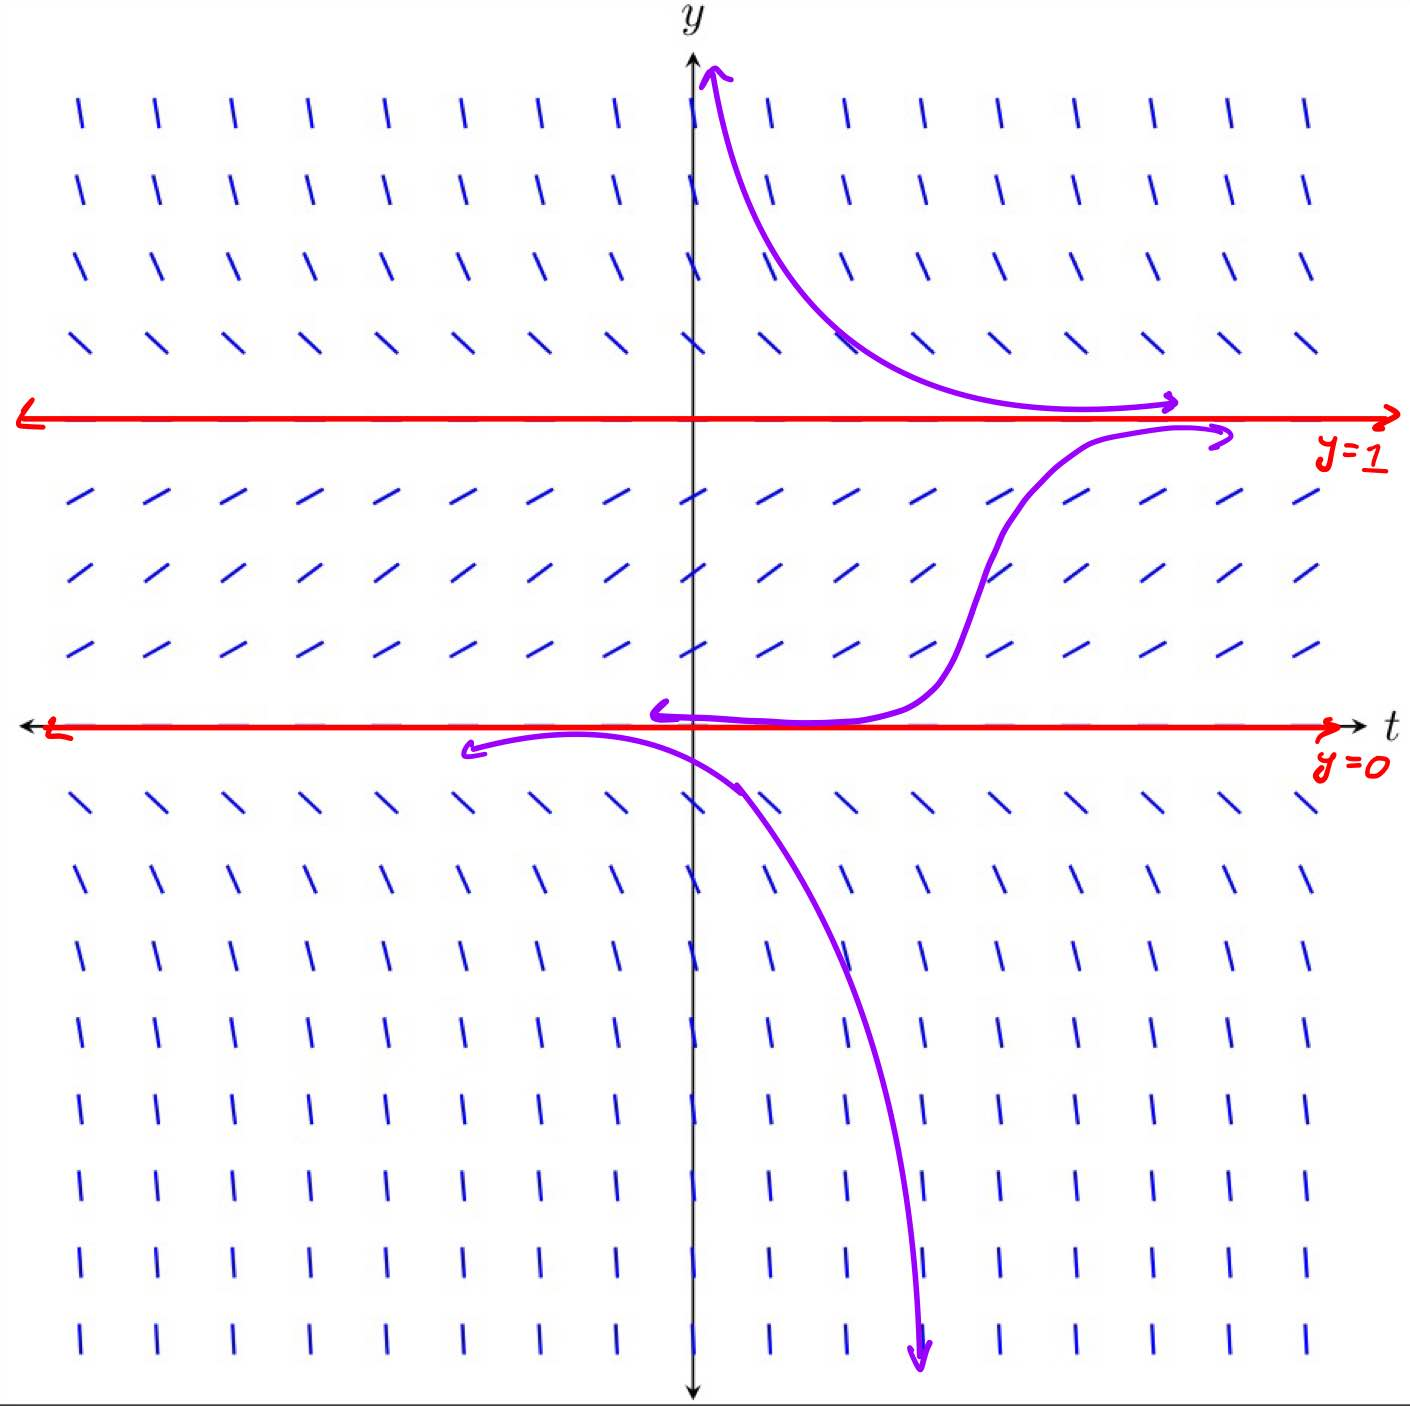
\includegraphics[scale=0.2]{image0.jpg}
\end{center}
When $y(0)=\frac{1}{2}$, $y$ will increase as $t$ increases. It starts out increasing at its maximum rate, and continutes to increase slower and slower as $t\to \infty$, with
\[
	\lim_{t \to \infty} y(t)=1
.\]
\end{soln}
\section*{Section 1.3 Problem 11}
\begin{soln}
	Since $f(t,y)$ is continuous, we can conclude that the slope field for $y\leq 3$ will be negative for at least some finite interval, and will either approach and asymptote off at an unknown equilibium point, or will continue to increase as it goes to infinity. Assuming the latter is true, for any $y(0)<3$, $y$ will go to infinity as $t$ goes to infinity. However, it's possible an equilibrium point $y_0(t)=0$ exists, in which case $y$ can only approach $y_0$ as $t\to \infty$.
\end{soln}
\section*{Section 1.3 Problem 14}
\begin{soln}
	\begin{center}	
	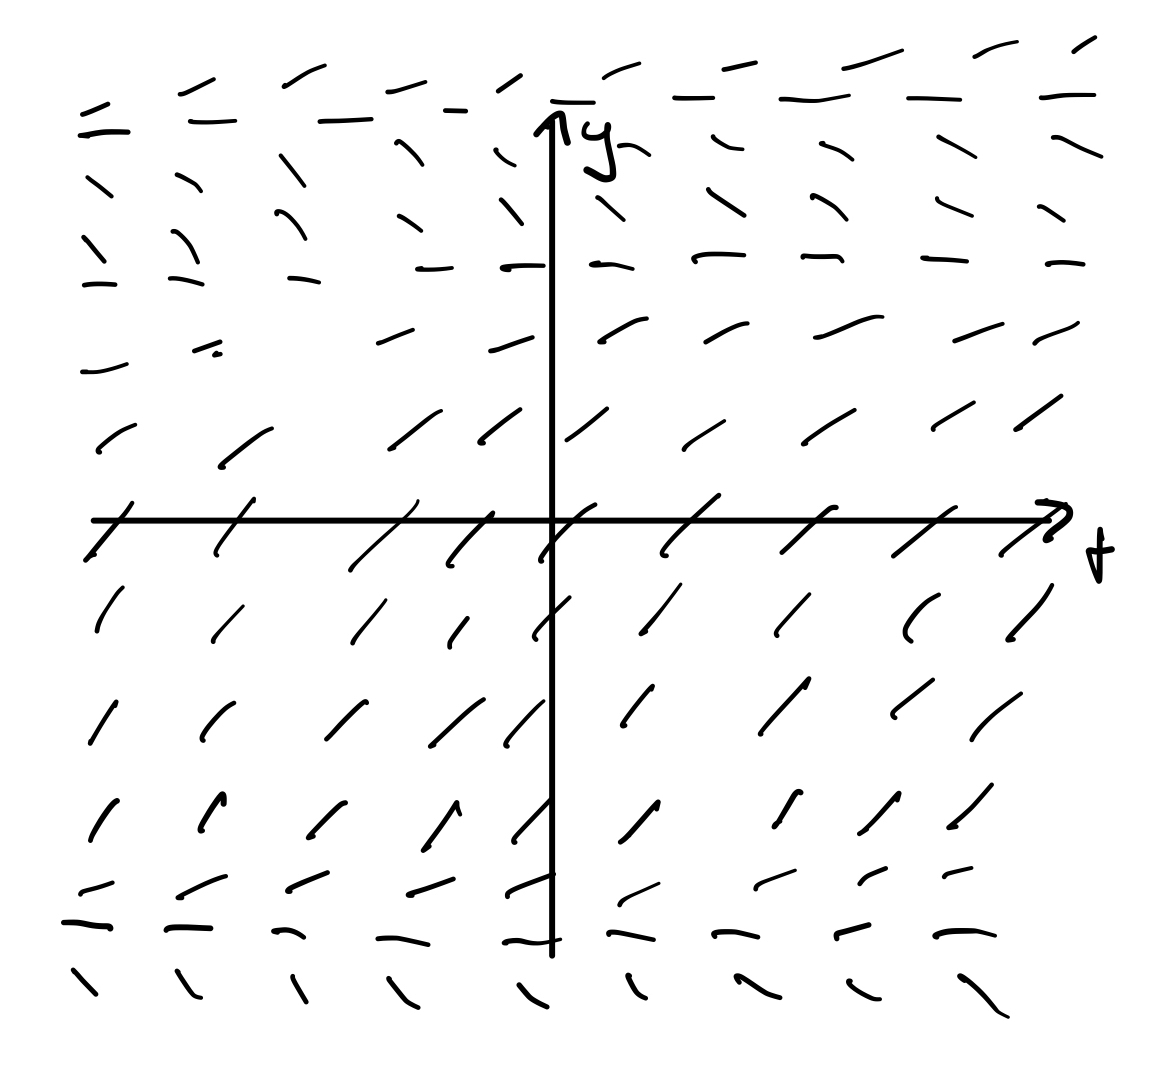
\includegraphics[scale=0.2]{image1.jpeg}	
	\end{center}
\end{soln}
\section*{Section 1.3 Problem 19}
The spiking of a neutron can be modeled as
\[
	\frac{\mathrm{d}\theta }{\mathrm{d}t} =1-\cos \theta +\left( 1+\cos \theta  \right) I(t)
\]
for some function $I(t)$, often a constant $I$. When $\theta =(2n+1)\pi $ for integer $n$, the neutron spikes. Equilibrium points here are values of $\theta $ where $\theta '=0$ for all $t$, and thus $\theta $ remains constant for all $t$. Since the function is only depedent on $t$ via $I(t)$ which is taken to be constant, we need only find the zeroes of $\theta '$ for some $I$.

\begin{soln}
	(b) To find the equilibrium points for the model, we need to find the zeroes of $\theta '$ for the given values of $I$, since the function $\theta '$ depends only on $\theta $ since $I(t)$ is taken to be constant. For an arbitrary constant $I$, let
	\[
		\frac{\mathrm{d}\theta }{\mathrm{d}t} =0
	.\]
	We have
	\begin{align*}
		1-\cos \theta +I\left( 1+\cos \theta  \right) &=0\\
		1-\cos \theta +I+I\cos \theta &=0\\
		(1+I)+\left( I\cos \theta -\cos \theta  \right) &=0\\
		\left( 1+I \right) +\left( I-1 \right)\cos \theta  &=0\\
		\cos \theta &=\frac{I+1}{I-1}
	,\end{align*}
	provided $I\neq 1$. Since we are testing values for $I$ that are not equal to 1, I don't think a full explanation of how I plugged in numbers and took the arccos to get the solutions is necessary. I used a calculator for $I_1$ and $I_3$, and $I_2$ was extremely easy. Due to how cosine works, for any solution $\theta $ I list, $2\pi n +\theta $ is also a solution for all $n\in\mathbb{Z}$. If $I=-0.1$, then $\theta \in \left\{ \arccos \left( \frac{1-0.1}{-0.1-1} \right) ,2\pi -\arccos \left( \frac{1-0.1}{-1-0.1} \right)  \right\} $ are equilibrium points.
	\[
		\arccos \left( \frac{1-0.1}{-1-0.1} \right) \approx 2.529
	.\]
	\[
		2\pi -\arccos \left( \frac{1-0.1}{-1-0.1} \right) \approx 3.754
	.\]
	If $I=0$, obviously $\frac{1}{-1}=-1$, and for $\cos \theta =-1$, $\theta =\pi $. Therefore, $\theta =\pi $ is the equilibrium point.

	If $I=0.1$, then $\theta \in\left\{ \arccos \left( \frac{1+0.1}{0.1-1} \right) , 2\pi -\arccos \left( \frac{0.1+1}{0.1-1} \right)  \right\} $ are equilibrium points. These values are all complex numbers, so there exist no $\theta \in\mathbb{R}$ such that $\theta $ is an equilibrium point. In other words, no equilibrium points exist unless for some reason you are using complex numbers.
\end{soln}
\section*{Section 1.4 Problem 2}
\begin{soln}
	\begin{center}
	\begin{tabular}{c|c}
		$t$ &$y$ \\
		\hline
		0&1\\
		0.25&0.75\\
		0.5&0.671875\\
		0.75&0.68402099609375\\
		1.0&0.7545498153194785
	\end{tabular}\\\vspace*{10pt}
	\begin{tikzpicture}
		\begin{axis}[
    xlabel={$t$},
    ylabel={$y$},
    xmin=0, xmax=1,
    ymin=0, ymax=1,
    ymajorgrids=true,
    xmajorgrids=true,
    grid style=dashed,
]

\addplot[
    color=blue,
    mark=*,
    ]
    coordinates {
    (0,1)(0.25,0.75)(0.5,0.672)(0.75,0.684)(1,0.755)
    };
    
\end{axis}
	\end{tikzpicture}
	\end{center}
\end{soln}
\section*{Section 1.4 Problem 6}
\begin{soln}
	\begin{center}
	\begin{tabular}{c|c}
		$t$ &$y$ \\
		\hline
		0&4\\
		1&-1\\
		2&-1\\
		3&-1\\
		4&-1\\
		5&-1
	\end{tabular}\\\vspace*{10pt}
	\begin{tikzpicture}
		\begin{axis}[
    xlabel={$t$},
    ylabel={$y$},
    xmin=0, xmax=5,
    ymin=-2, ymax=4,
    ymajorgrids=true,
    xmajorgrids=true,
    grid style=dashed,
]

\addplot[
    color=blue,
    mark=*,
    ]
    coordinates {
    (0,4)(1,-1)(2,-1)(3,-1)(4,-1)(5,-1)
    };
    
\end{axis}
	\end{tikzpicture}
	\end{center}
\end{soln}
\newpage
\section*{Section 1.4 Problem 9}
\begin{soln}
	\begin{center}
		\begin{tabular}{c|c}
			$t$ &$y$ \\
			\hline
			0&0.2\\
0.1&0.20320000000000002\\
0.2&0.20649000632320003\\
0.3&0.20987338397150784\\
0.4&0.213353641821741\\
0.5&0.21693443846093888\\
0.6&0.22061958810837687\\
0.7&0.2244130665942669\\
0.8&0.22831901735827956\\
0.9&0.23234175742306212\\
   1.0&0.2364857832887022\\
1.1&0.24075577668342468\\
1.2&0.2451566100935247\\
1.3&0.24969335198142228\\
1.4&0.2543712715845504\\
1.5&0.2591958431693169\\
1.6&0.26417274959335046\\
1.7&0.26930788500538877\\
1.8&0.27460735648520596\\
1.9&0.2800774843956438\\
2.0&0.28572480118482907\\
2.1&0.2915560483387995\\
2.2&0.2975781711428217\\
2.3&0.30379831086354936\\
2.4&0.3102237939138147\\
2.5&0.3168621175074011\\
2.6&0.3237209312529289\\
2.7&0.33080801407459204\\
2.8&0.33813124578383075\\
2.9&0.3456985725614776\\
3.0&0.3535179655463773\\
3.1&0.36159737166652356\\
3.2&0.36994465579576413\\
3.3&0.3785675332774428\\
3.4&0.3874734918314334\\
3.5&0.3966697018596087\\
3.6&0.4061629141949977\\
3.7&0.4159593444113306\\
3.8&0.4260645429334345\\
3.9&0.43648325037751085\\
4.0&0.44721923781726286\\
		\end{tabular}
		\begin{tabular}{c|c}
			\hline
4.1&0.4582751320313395\\
4.2&0.4696522262536094\\
4.3&0.4813502775330185\\
4.4&0.49336729252394246\\
4.5&0.5056993043757608\\
4.6&0.5183401443691159\\
4.7&0.5312812130428315\\
4.8&0.5445112567430355\\
4.9&0.5580161567612277\\
5.0&0.5717787394480452\\
5.1&0.5857786168104478\\
5.2&0.599992068017248\\
5.3&0.6143919728284217\\
5.4&0.6289478080924873\\
5.5&0.6436257179864621\\
5.6&0.6583886674798007\\
5.7&0.6731966864927752\\
5.8&0.6880072093469357\\
5.9&0.7027755103972091\\
   6.0&0.7174552323059498\\
6.1&0.7319989984799932\\
6.2&0.7463590960488811\\
6.3&0.7604882108017152\\
6.4&0.7743401911554455\\
6.5&0.7878708149358706\\
6.6&0.8010385309007679\\
6.7&0.8138051468034325\\
6.8&0.8261364375134088\\
6.9&0.8380026502267746\\
7.0&0.8493788888719632\\
7.1&0.8602453660454099\\
7.2&0.8705875176732772\\
7.3&0.880395982516577\\
7.4&0.8896664550594812\\
7.5&0.8983994257688731\\
7.6&0.9065998268430375\\
7.7&0.914276604193148\\
7.8&0.9214422374985565\\
7.9&0.9281122298640405\\
8.0&0.9343045871106501\\
\end{tabular}
\begin{tabular}{c|c}
			\hline
8.1&0.9400393043442943\\
8.2&0.9453378744842706\\
8.3&0.9502228302013387\\
8.4&0.9547173274756139\\
8.5&0.9588447759463803\\
8.6&0.9626285185345882\\
8.7&0.9660915605600928\\
8.8&0.9692563467832646\\
8.9&0.972144583466991\\
   9.0&0.9747771016435095\\
9.1&0.9771737572260351\\
9.2&0.9793533633641218\\
9.3&0.9813336504391031\\
9.4&0.983131249270489\\
9.5&0.9847616934015219\\
9.6&0.9862394367063757\\
9.7&0.9875778829758413\\
9.8&0.9887894245644197\\
9.9&0.989885487598809\\
10.0&0.9908765816415668\\
\end{tabular}
	\end{center}
	\begin{center}
	\begin{tikzpicture}
		\begin{axis}[
    xlabel={$t$},
    ylabel={$y$},
    xmin=0, xmax=10,
    ymin=0, ymax=1,
    ymajorgrids=true,
    xmajorgrids=true,
    grid style=dashed,
]

\addplot[
    color=blue,
    mark=*,
    samples=1000
    ]
    coordinates {
	    (0,0.2)(0.1,0.20320000000000002)(0.2,0.20649000632320003)(0.30000000000000004,0.20987338397150784)(0.4,0.213353641821741)(0.5,0.21693443846093888)(0.6,0.22061958810837687)(0.7,0.2244130665942669)(0.7999999999999999,0.22831901735827956)(0.8999999999999999,0.23234175742306212)(0.9999999999999999,0.2364857832887022)(1.0999999999999999,0.24075577668342468)(1.2,0.2451566100935247)(1.3,0.24969335198142228)(1.4000000000000001,0.2543712715845504)(1.5000000000000002,0.2591958431693169)(1.6000000000000003,0.26417274959335046)(1.7000000000000004,0.26930788500538877)(1.8000000000000005,0.27460735648520596)(1.9000000000000006,0.2800774843956438)(2.0000000000000004,0.28572480118482907)(2.1000000000000005,0.2915560483387995)(2.2000000000000006,0.2975781711428217)(2.3000000000000007,0.30379831086354936)(2.400000000000001,0.3102237939138147)(2.500000000000001,0.3168621175074011)(2.600000000000001,0.3237209312529289)(2.700000000000001,0.33080801407459204)(2.800000000000001,0.33813124578383075)(2.9000000000000012,0.3456985725614776)(3.0000000000000013,0.3535179655463773)(3.1000000000000014,0.36159737166652356)(3.2000000000000015,0.36994465579576413)(3.3000000000000016,0.3785675332774428)(3.4000000000000017,0.3874734918314334)(3.5000000000000018,0.3966697018596087)(3.600000000000002,0.4061629141949977)(3.700000000000002,0.4159593444113306)(3.800000000000002,0.4260645429334345)(3.900000000000002,0.43648325037751085)(4.000000000000002,0.44721923781726286)(4.100000000000001,0.4582751320313395)(4.200000000000001,0.4696522262536094)(4.300000000000001,0.4813502775330185)(4.4,0.49336729252394246)(4.5,0.5056993043757608)(4.6,0.5183401443691159)(4.699999999999999,0.5312812130428315)(4.799999999999999,0.5445112567430355)(4.899999999999999,0.5580161567612277)(4.999999999999998,0.5717787394480452)(5.099999999999998,0.5857786168104478)(5.1999999999999975,0.599992068017248)(5.299999999999997,0.6143919728284217)(5.399999999999997,0.6289478080924873)(5.4999999999999964,0.6436257179864621)(5.599999999999996,0.6583886674798007)(5.699999999999996,0.6731966864927752)(5.799999999999995,0.6880072093469357)(5.899999999999995,0.7027755103972091)(5.999999999999995,0.7174552323059498)(6.099999999999994,0.7319989984799932)(6.199999999999994,0.7463590960488811)(6.299999999999994,0.7604882108017152)(6.399999999999993,0.7743401911554455)(6.499999999999993,0.7878708149358706)(6.5999999999999925,0.8010385309007679)(6.699999999999992,0.8138051468034325)(6.799999999999992,0.8261364375134088)(6.8999999999999915,0.8380026502267746)(6.999999999999991,0.8493788888719632)(7.099999999999991,0.8602453660454099)(7.19999999999999,0.8705875176732772)(7.29999999999999,0.880395982516577)(7.39999999999999,0.8896664550594812)(7.499999999999989,0.8983994257688731)(7.599999999999989,0.9065998268430375)(7.699999999999989,0.914276604193148)(7.799999999999988,0.9214422374985565)(7.899999999999988,0.9281122298640405)(7.999999999999988,0.9343045871106501)(8.099999999999987,0.9400393043442943)(8.199999999999987,0.9453378744842706)(8.299999999999986,0.9502228302013387)(8.399999999999986,0.9547173274756139)(8.499999999999986,0.9588447759463803)(8.599999999999985,0.9626285185345882)(8.699999999999985,0.9660915605600928)(8.799999999999985,0.9692563467832646)(8.899999999999984,0.972144583466991)(8.999999999999984,0.9747771016435095)(9.099999999999984,0.9771737572260351)(9.199999999999983,0.9793533633641218)(9.299999999999983,0.9813336504391031)(9.399999999999983,0.983131249270489)(9.499999999999982,0.9847616934015219)(9.599999999999982,0.9862394367063757)(9.699999999999982,0.9875778829758413)(9.799999999999981,0.9887894245644197)(9.89999999999998,0.989885487598809)(9.99999999999998,0.9908765816415668)

    };
    
\end{axis}
	\end{tikzpicture}
	\end{center}
\end{soln}
\section*{Section 1.5, Problem 4}
\begin{soln}
	Since Picard's theorem applies for all $(t,y)$, we know that for any point $(t_0,y_0)$ on a solution $y_1$, the solution $y_1$ must be unique within a neighborhood of $(t_0,y_0)$. The functions being continuous allows us to generalize this and state that if $y,y_1$ are \emph{distinct} solutions for different intitial values, then there is no $t$ such that $y_1(t)=y(t)$. Since $y_1(0)=-1$ and $y_2(0)=1$, we have $y_1(0)<y(0)<y_2(y)$, and thus $y_1(t)<y(t)<y_2(t)$ for all $t$.
\end{soln}
\section*{Section 1.5, Problem 15}
\begin{soln}
	\begin{align*}
		&\qquad \frac{\mathrm{d}y}{\mathrm{d}t} =\left( y+2 \right) ^{-2}\\
		&\implies \int \left( y+2 \right) ^{2} \,\mathrm{d} y=t+C\\
		&\implies \frac{\left( y+2 \right) ^3}{3}=t+C\\
		&\implies y=\sqrt[3]{3t+C}-2 \\
		&\qquad y(0)=1\\
		&\implies \sqrt[3]{C}=3\\
		&\implies C=27\\
		&\implies y=\sqrt[3]{3t+27}-2 
	.\end{align*}
	The derivative is discontinuous at $y-2$, which happens at $t=-9$. Thus, Picard's theorem is not satisfied for $t=-9$, so the solution will only exist for $t\in[-9,\infty)$. As $t\to -9$, the derivative approaches infinity.
\end{soln}
\section*{Supplimental Problem 1}
\begin{soln}
	\begin{align*}
		\frac{\mathrm{d}y}{\mathrm{d}t} (t_0)&\approx \frac{y(t_0+\Delta t)-y)(t_0-\Delta t)}{2\Delta t}\\
		2\Delta t \frac{\mathrm{d}y}{\mathrm{d}t}(t_0) +y(t_0-\Delta t)&\approx y(t_0+\Delta t)
	.\end{align*}
	We can apply this similarly to Euler's method by rewriting it as
	\[
		2\Delta t \frac{\mathrm{d}y}{\mathrm{d}t} (t_0+\Delta t)+y(t_0)=y(t_0+2\Delta t)
	.\]
	We can use the classic Euler's method to obtain $y(t_0+\Delta t)$, and plug this into $\frac{\mathrm{d}y}{\mathrm{d}t} $ to obtain an approximation for $y(t_0+2\Delta t)$. We can then slide our approximation of $y(t_0+\Delta t)$ back to where $y(t_0)$ was, and slide $y(t_0+2\Delta t)$ to where $y(t_0+\Delta t)$ was, and thus we have an Eulerian approximation schema from the center difference approximation.
	\begin{lstlisting}[language=python]
#!/usr/bin/env python3

import matplotlib.pyplot as plt

# implement desired values here
t_0 = 0 # t_0 value
y_0 = 0.25 # y_0 value
t_step = 0.01 # t step
t_f = 5 # final t value

# implement desired diff eq here
def diffeq(y):
    return y * (1 - y)

# implements the centered difference euler approximation method
def centered_euler(y_k, y_kk, delta_t):
    return y_kk + (diffeq(y_k)*2*delta_t)

# generates a list of t values
t_vals = []
t = t_0
while t <= t_f:
    t_vals.append(t)
    t += t_step

# generates the first y value via euler's method
y_vals = [y_0]
y_vals.append(y_0 + (t_step * diffeq(y_0)))
# generates the remaining y values
for t in t_vals[2:]:
    y_vals.append(centered_euler(y_vals[len(y_vals)-1], y_vals[len(y_vals) - 2],
    t_step))

# prints the results to console because i wanted it to, feel free to remove
for i in range(len(t_vals)):
    print(f"({t_vals[i]},{y_vals[i]})")

# plotting the results
plt.scatter(t_vals, y_vals, label="circles", color="blue", s=30)
plt.xlabel('t')
plt.ylabel('y')
plt.title('Center Difference Euler Method Approximation')
plt.show()

	\end{lstlisting}
	I'm a horrible programmer. I also wrote code for the regular Euler's method, and plotted both of them against each other for \verb|t_step| = 0.1 and 0.01. I have no idea why one of the graphs is shorter than the others.
	\begin{center}
		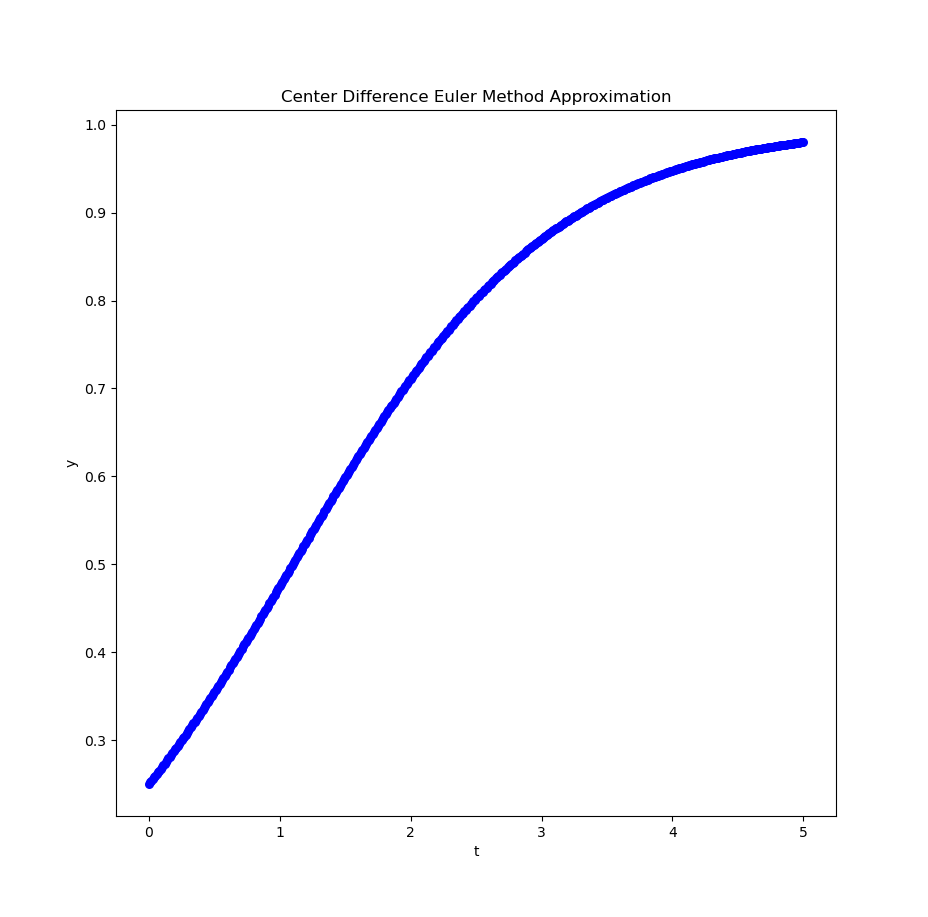
\includegraphics[scale=0.35]{CenterEuler.png}
		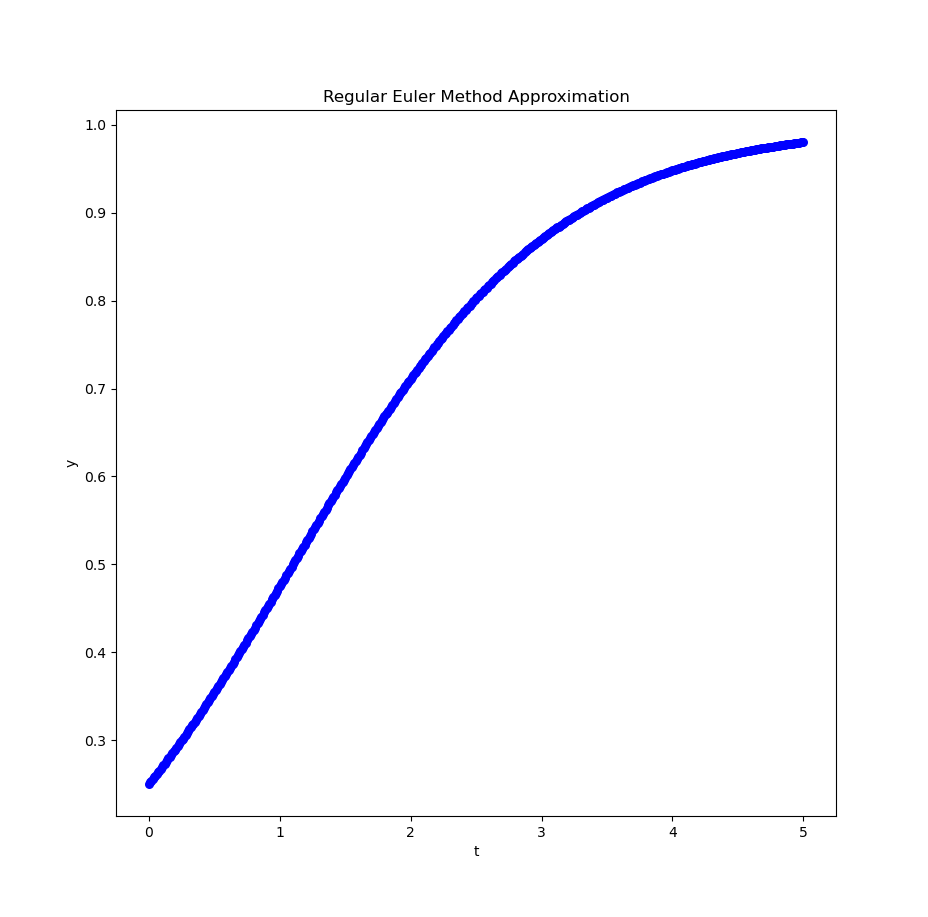
\includegraphics[scale=0.35]{Euler.png}
	\end{center}
	\begin{center}
		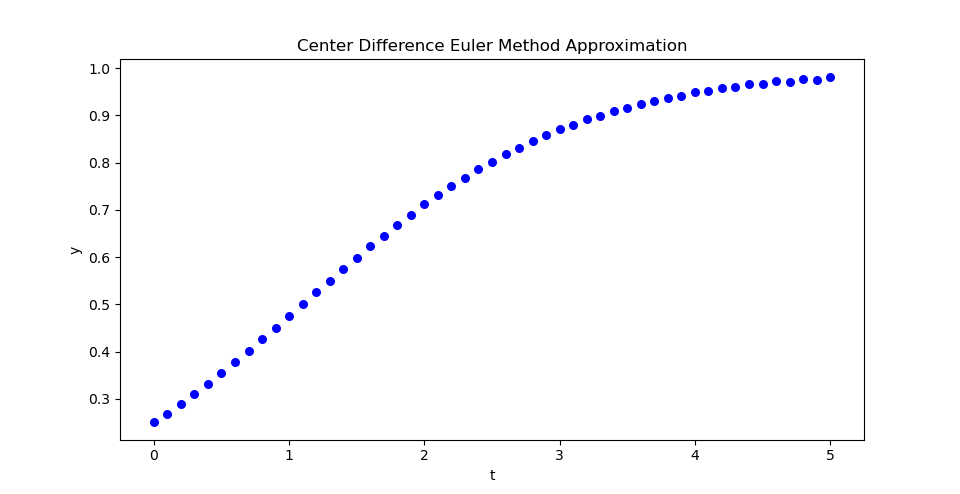
\includegraphics[scale=0.35]{BigEulerCenter.png}
		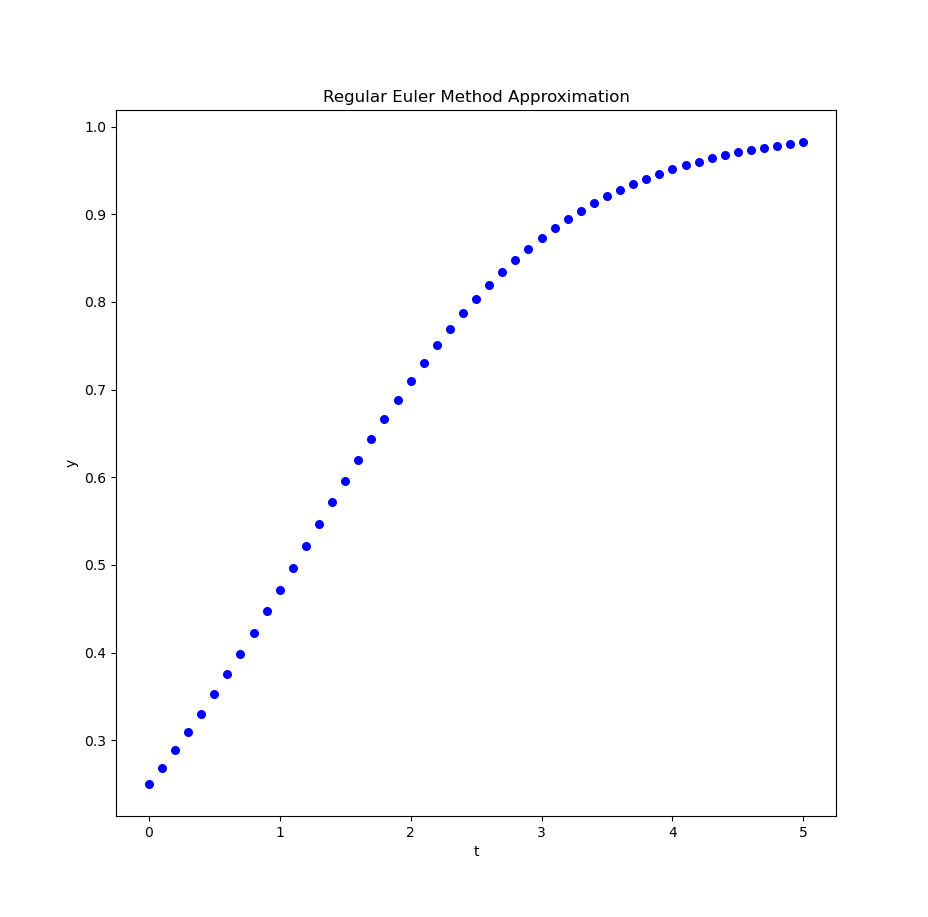
\includegraphics[scale=0.35]{BigEuler.png}
	\end{center}
	It appears the center difference approximation method is slightly more accurate than the classic Euler's method from this visual depiction, especially for small values of $\Delta t$.
\end{soln}
\section*{Supplimental Problem 2}
\begin{soln}
	\begin{center}
		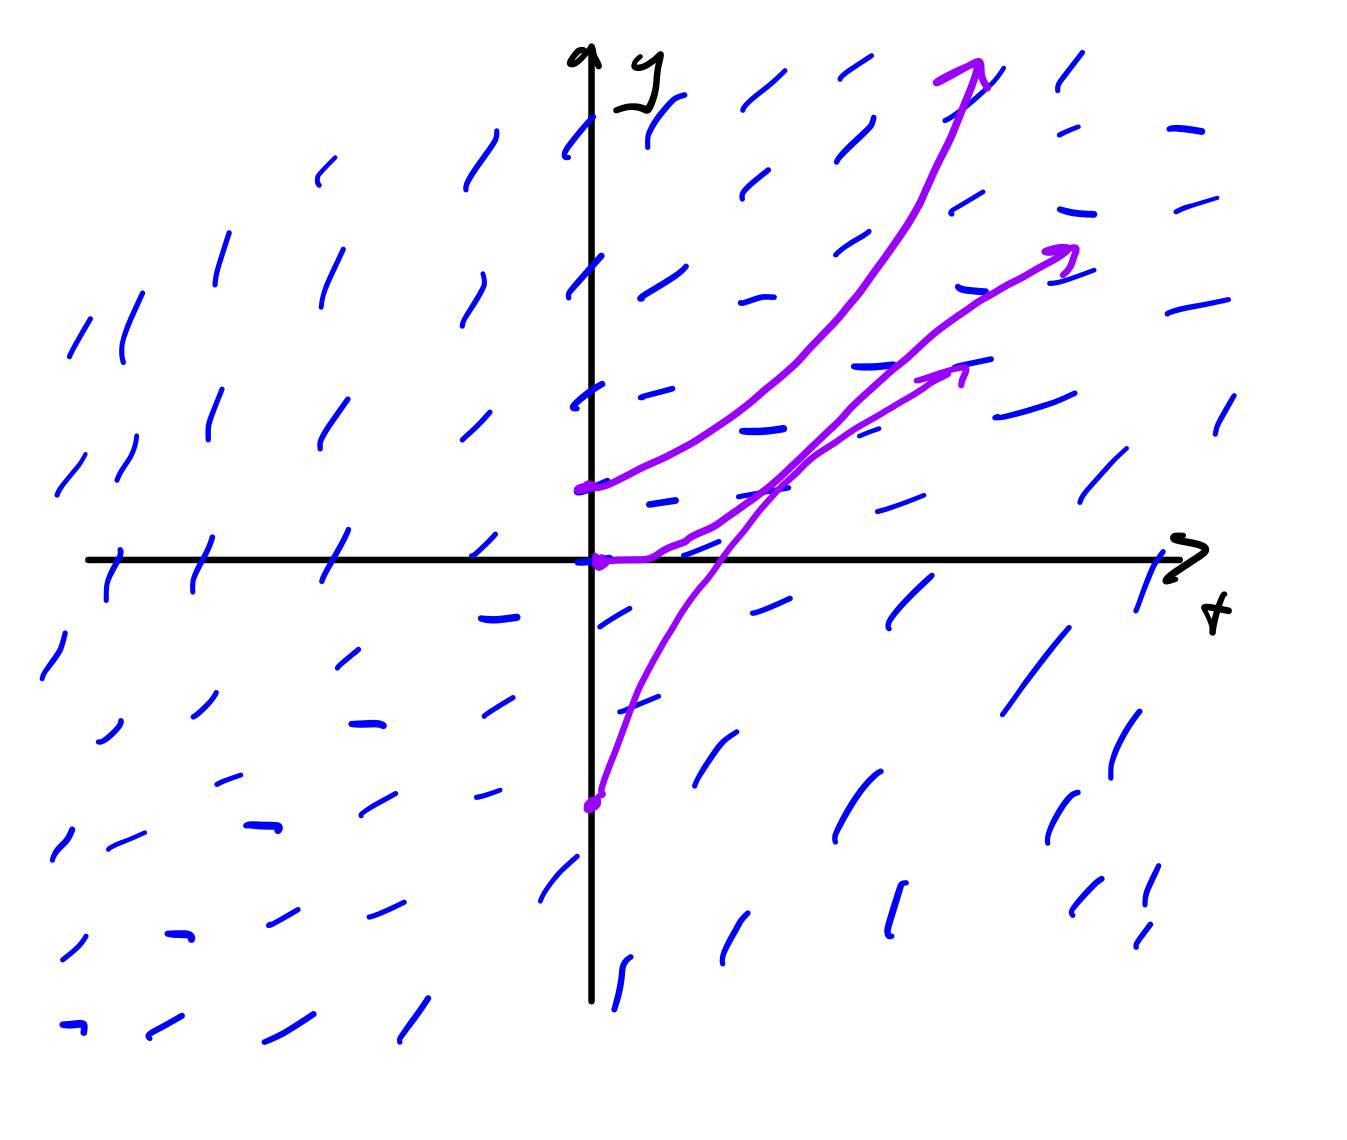
\includegraphics[scale=0.3]{slowo.jpg}
	\end{center}
	For a solution to the IVP with $y_0 < 0$, our solution $y$ will approach the line $y=t$, and will asymptote off without reaching it. So as $t\to \infty$, $y\to t$. This is because the slope is still positive below $y=t$, but it is decreasingly so, and the slope at $y=t$ is 0.

	Using Euler's method, I obtained the following three graphs for their respectiveee values of $y_0$.
	\begin{center}
		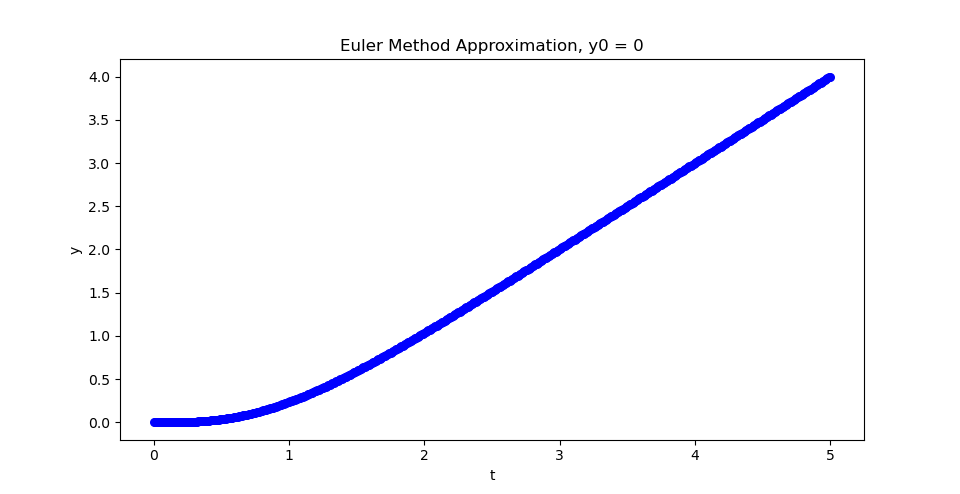
\includegraphics[scale=0.5]{SuperEuler.png}
		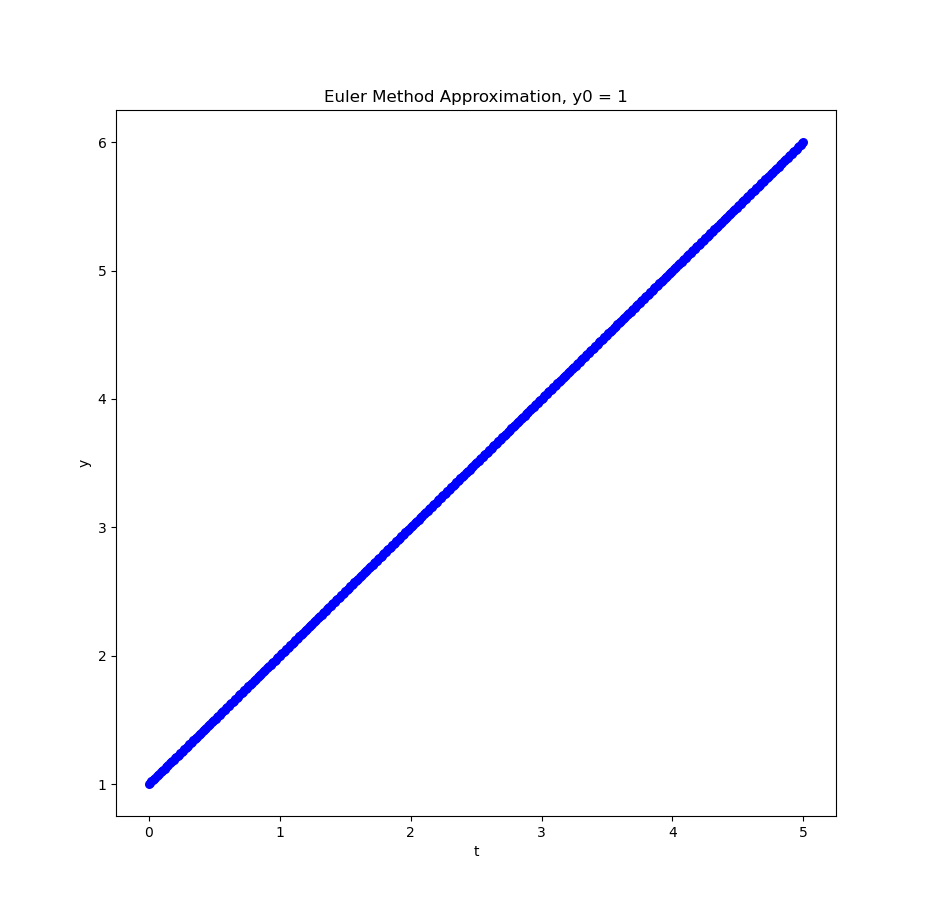
\includegraphics[scale=0.5]{SuperEuler1.png}
		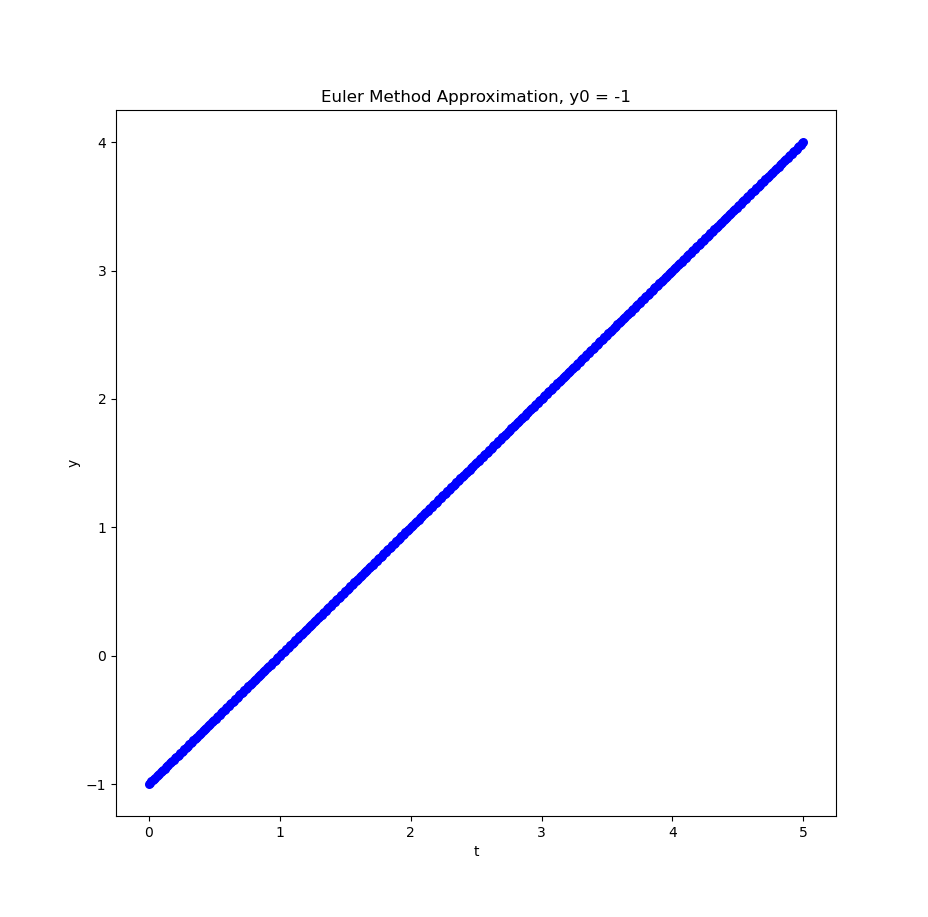
\includegraphics[scale=0.5]{SuperEuler11.png}
	\end{center}
	The function appears to have the functions $y=t\pm 1$ as solutions, which I happened to check out of pure luck. Plugging in, we have
	\[
		\frac{\mathrm{d}y}{\mathrm{d}t} \left( t\pm1 \right) =1
	.\]
	\[
		(y_+-t)^2 = (t+1-t)^2 = 1^2 = 1 = \frac{\mathrm{d}y}{\mathrm{d}t} 
	.\]
	\[
		(y_- -t)^2 = (t-1-t)^2 = (-1)^2 = 1 = \frac{\mathrm{d}y}{\mathrm{d}t} 
	.\]
	However, finding a general solution does not look simple given these two solutions.

	The assignment is due in 10 minutes omg

\begin{align*}
	\frac{\mathrm{d}y}{\mathrm{d}t} &=\left( y-t \right) ^2\\
	\text{Let }u&=y-t\\
	\implies \frac{\mathrm{d}u}{\mathrm{d}t} &=\frac{d}{dt}(y-t)=\frac{\mathrm{d}y}{\mathrm{d}t} -1\\
	\implies \frac{\mathrm{d}u}{\mathrm{d}t} -1 &= \frac{\mathrm{d}y}{\mathrm{d}t} \\
	\implies \frac{\mathrm{d}u}{\mathrm{d}t} +1&=u^2\\
	\implies \frac{\mathrm{d}u}{\mathrm{d}t} &=u^2 - 1\\
	\implies \int \frac{1}{u^2-1}\frac{\mathrm{d}u}{\mathrm{d}t}  \,\mathrm{d} t&=t+C\\
	\implies \int \frac{1}{u^2-1} \,\mathrm{d} u&=t+C\\
	\int \frac{1}{u^2-1} \,\mathrm{d} u&=\int \frac{1}{u+1}\frac{1}{u-1} \,\mathrm{d} u\\
					   &=\int \frac{0.5}{u-1}-\frac{0.5}{u+1} \,\mathrm{d} u\\
					   &=\frac{1}{2}\int \frac{1}{u-1}-\frac{1}{u+1} \,\mathrm{d} u\\
					   &=\frac{1}{2}\left( \ln \left| u-1 \right| -\ln \left| u+1 \right|  \right)\\
					   &=\frac{1}{2}\ln \left| \frac{u-1}{u+1} \right| 
.\end{align*}
I've done this integral bfore and made the EXACT SAME MISTAKE I DONT KNOW WHAT IT IS but it should be
\[
	t+C = \frac{1}{2}\ln \left| \frac{1-u}{1+u} \right| 
.\]
It follows that
\[
	e^{t}e^{C}=\frac{1-u}{1+u}
.\]
\begin{align*}
	&\qquad\left( 1+u \right) \left( e^{t}e^{C} \right) =1-u\\
	&\implies e^te^C + u\left( 1+e^te^C \right) =1\\
	&\implies u=\frac{1-e^te^C}{1+e^te^C}\\
	&\implies y=\frac{1-e^te^C}{1+e^te^C}+t
.\end{align*}
This solution makes a lot more sense because  you see  $y=t$ if the mess of exponentials equals $0$, but it is obviously never going to stay at $0$. But plugging in 1 or -1 for $t$ will obviously give stable behavior. Idk I have 4 minutes to submit so thats my analysis.
\end{soln}
\end{document}
